\documentclass{article}
\usepackage{fullpage}
\usepackage[utf8]{inputenc}
\usepackage{pict2e}
\usepackage{amsmath}
\usepackage{enumitem}
\usepackage{eurosym}
\usepackage{mathtools}
\usepackage{amssymb, amsfonts, latexsym, cancel}
\setlength{\parskip}{0.3cm}
\usepackage{graphicx}
\usepackage{fontenc}
\usepackage{slashbox}
\usepackage{setspace}
\usepackage{gensymb}
\usepackage{accents}
\usepackage{adjustbox}
\setstretch{1.35}
\usepackage{bold-extra}
\usepackage[document]{ragged2e}
\usepackage{subcaption}
\usepackage{tcolorbox}
\usepackage{xcolor, colortbl}
\usepackage{wrapfig}
\usepackage{empheq}
\usepackage{array}
\usepackage{parskip}
\usepackage{arydshln}
\graphicspath{ {images/} }
\renewcommand*\contentsname{\color{black}Índice} 
\usepackage{array, multirow, multicol}
\definecolor{lightblue}{HTML}{007AFF}
\usepackage{color}
\usepackage{etoolbox}
\usepackage{listings}
\usepackage{mdframed}
\setlength{\parindent}{0pt}
\usepackage{underscore}
\usepackage{hyperref}
\usepackage{tikz}
\usepackage{tikz-cd}
\usetikzlibrary{shapes, positioning, patterns}
\usepackage{tikz-qtree}
\usepackage{biblatex}
\usepackage{pdfpages}
\usepackage{pgfplots}
\usepackage{pgfkeys}
\addbibresource{biblatex-examples.bib}
\usepackage[a4paper, left=1cm, right=1cm, top=1cm,
bottom=1.5cm]{geometry}
\usepackage{titlesec}
\usepackage{titletoc}
\usepackage{tikz-3dplot}
\usepackage{kbordermatrix}
\usetikzlibrary{decorations.pathreplacing}
\newcommand{\Ej}{\textcolor{lightblue}{\underline{Ejemplo}}}
\setlength{\fboxrule}{1.5pt}

% Configura el formato de las secciones utilizando titlesec
\titleformat{\section}
{\color{red}\normalfont\LARGE\bfseries}
{Tema \thesection:}
{10 pt}
{}

% Ajusta el formato de las entradas de la tabla de contenidos
\addtocontents{toc}{\protect\setcounter{tocdepth}{4}}
\addtocontents{toc}{\color{black}}

\titleformat{\subsection}
{\normalfont\Large\bfseries\color{red}}{\thesubsection)}{1em}{\color{lightblue}}

\titleformat{\subsubsection}
{\normalfont\large\bfseries\color{red}}{\thesubsubsection)}{1em}{\color{lightblue}}

\newcommand{\bboxed}[1]{\fcolorbox{lightblue}{lightblue!10}{$#1$}}
\newcommand{\rboxed}[1]{\fcolorbox{red}{red!10}{$#1$}}

\DeclareMathOperator{\N}{\mathbb{N}}
\DeclareMathOperator{\Z}{\mathbb{Z}}
\DeclareMathOperator{\R}{\mathbb{R}}
\DeclareMathOperator{\Q}{\mathbb{Q}}
\DeclareMathOperator{\K}{\mathbb{K}}
\DeclareMathOperator{\im}{\imath}
\DeclareMathOperator{\jm}{\jmath}
\DeclareMathOperator{\col}{\mathrm{Col}}
\DeclareMathOperator{\fil}{\mathrm{Fil}}
\DeclareMathOperator{\rg}{\mathrm{rg}}
\DeclareMathOperator{\nuc}{\mathrm{nuc}}
\DeclareMathOperator{\dimf}{\mathrm{dimFil}}
\DeclareMathOperator{\dimc}{\mathrm{dimCol}}
\DeclareMathOperator{\dimn}{\mathrm{dimnuc}}
\DeclareMathOperator{\dimr}{\mathrm{dimrg}}
\DeclareMathOperator{\dom}{\mathrm{Dom}}
\DeclareMathOperator{\infi}{\int_{-\infty}^{+\infty}}
\newcommand{\dint}[2]{\int_{#1}^{#2}}

\newcommand{\bu}[1]{\textcolor{lightblue}{\underline{#1}}}
\newcommand{\lb}[1]{\textcolor{lightblue}{#1}}
\newcommand{\db}[1]{\textcolor{blue}{#1}}
\newcommand{\rc}[1]{\textcolor{red}{#1}}
\newcommand{\tr}{^\intercal}

\renewcommand{\CancelColor}{\color{lightblue}}

\newcommand{\dx}{\:\mathrm{d}x}
\newcommand{\dt}{\:\mathrm{d}t}
\newcommand{\dy}{\:\mathrm{d}y}
\newcommand{\dz}{\:\mathrm{d}z}
\newcommand{\dth}{\:\mathrm{d}\theta}
\newcommand{\dr}{\:\mathrm{d}\rho}
\newcommand{\du}{\:\mathrm{d}u}
\newcommand{\dv}{\:\mathrm{d}v}
\newcommand{\tozero}[1]{\cancelto{0}{#1}}
\newcommand{\lbb}[2]{\textcolor{lightblue}{\underbracket[1pt]{\textcolor{black}{#1}}_{#2}}}
\newcommand{\dbb}[2]{\textcolor{blue}{\underbracket[1pt]{\textcolor{black}{#1}}_{#2}}}
\newcommand{\rub}[2]{\textcolor{red}{\underbracket[1pt]{\textcolor{black}{#1}}_{#2}}}

\author{Francisco Javier Mercader Martínez}
\date{}
\renewcommand{\arraystretch}{1}
\setlength{\arraycolsep}{6pt}

\title{Álgebra Lineal\\Ejercicios Tema 4: Subespacios vectoriales, bases y coordenadas}

\begin{document}
\maketitle
\begin{enumerate}[label=\color{red}\textbf{\arabic*)}]
    \item \lb{Determina cuáles de ls siguientes subonjunto de $\R^3$ son subespacios vectoriales:}
        \begin{enumerate}[label=\color{red}\textbf{\alph*)}]
            \item \db{$\{(x,y,z|x=1)\} $} 

                No es un subespacio vectorial porque no contiene al $(0,0,0)$.
            \item \db{$\{(x,y,z)|xyz=0\} $} 

                $W=\{(x,y,z)|xyz=0\} $ 

                Tomamos $(x_1,y_1,z_1),(x_2,y_2,z_2)\in W\longrightarrow \underbrace{(x_1,y_1,z_1)+(x_2,y_2,z_2)}_{(x_1+x_2,y_1+y_2,z_1+z_2)}\in W$ 

                $(x_1+x_2)\cdot (y_1+y_2)\cdot (z_1+z_2)=0$

                Claramente no es un subespacio vectorial porque \textit{"las tres componentes  están multiplicando"} 

                Para verlo más claramente: \[
                \begin{array}{l}
                    v_1=(1,1,0)\in W\text{ ya que }1\cdot 1\cdot 0=0\\
                    v_2=(0,0,1)\in W\text{ ya que }0\cdot 0\cdot 1=0
                \end{array}
                \]
                Sin embargo, $v_1+v_2=(1,1,1)\notin W$ ya que \[
                1\cdot 1\cdot 1=1\neq 0.
                \] 
            \item \db{$\{(x,y,z)|x+y+z=0\} $} 

                $(x_1,y_1,z_1),(x_2,y_2,z_2)\in W\longrightarrow (x_1+x_2,y_1+y_2,z_1+z_2)\in W$

                $(x_1+x_2)+(y_1+y_2)+(z_1+z_2)=\underbrace{(x_1+y_1+z_1)}_{=0}+\underbrace{(x_2+y_2+z_2)}_{=0}=0$

                Sean ahora $(x_1,y_1,z_1)\in W$ y $\alpha\in \R\longrightarrow \alpha(x_1,y_1,z_1)\in W$

                $\begin{array}{l}
                    \alpha(x_1,y_1,z_1)=(\alpha x_1,\alpha y_1,\alpha z_1)\\
                    \alpha x_1+\alpha y_1+\alpha z_1=\alpha\underbrace{(x_1+y_1+z_1)}_{=0}=0
                \end{array}$
        \end{enumerate}
    \item \lb{Comprueba que, en $\R^3$, el subespacio generado por los vectores $(1,2,1)$ y  $(6,1,-16)$ coincide con el subespacio generador por los vectores  $(-3,7,20)$ y  $(4,9,6)$.} 

        Para verificar si el subespacio generador po $\{(1,2,1),(6,1,-16)\} $ coincide con el generado por $\{(-3,7,20),(4,9,6)\} $ en $\R^3$, debemos comprobar si cada conjunto de vectores puede ser expresado como una combinación lineal de los vectores del otro conjunto. Esto implica que ambos subconjuntos generan el mismo campo vectorial.

        Paso a seguir:
        \begin{enumerate}[label=\arabic*)]
            \item \textbf{Matriz ampliada:} Consideramos todos los vectores como filas de una matriz y verificamos si los vectores de un conjunto son combinación lineal de los del otro. Esto se hace calculando las filas escalonadas (rango). \[
            A_1=\begin{bmatrix} 
                1 & 2 & 1\\
                6 & 1 & -16\\
                -3 & 7 & 20\\
                4 & 9 & 6
            \end{bmatrix} 
            \]  
            Reducimos la matriz a su forma escalonada para identificar si el rango es igual a 2 (dimensión de un plano en $\R^3$).
        \item \textbf{Dependencia lineal:} Si se confirma que el rango es 2, probamos si los vectores de un conjunto pertenecen al subespacio generado por los vectores del otro. Para esto, verificamos si existe una relación lineal. 

            $\begin{bmatrix} 
                1 & 2 & 1 \\
                6 & 1 & -16\\
                -3 & 7 & 20\\
                4 & 9 & 6
            \end{bmatrix}\xrightarrow[\begin{subarray}{l}
                F_3\to F_3+3F_1\\
                F_4\to F_4-4F_1
            \end{subarray}]{F_2\to F_2-6F_1}\begin{bmatrix} 
                1 & 2 & 1\\
                0 & -11 & -22\\
                0 & 13 & 23\\
                0 & 1 & 2
            \end{bmatrix}\xrightarrow{F_2\leftrightarrow F_4}\begin{bmatrix} 
                1 & 2 & 1\\
                0 & 1 & 2\\
                0 & 13 & 23\\
                0 & -11 & -22
            \end{bmatrix}\xrightarrow[\begin{subarray}{l}
                F_3\to F_3-13F_2\\
                F_4\to F_4-F_2
            \end{subarray}]{F_1\to F_1-2F_2}\begin{bmatrix} 
                1 & 0 & 3\\
                0 & 1 & 2\\
                0 & 0 & -3\\
                0 & 0 & 0
            \end{bmatrix}\xrightarrow{F_3\to -\frac{1}{3} F_3}\begin{bmatrix} 
                1 & 0 & -3\\
                0 & 1 & 2\\
                0 & 0 & 1\\
                0 & 0 & 0
            \end{bmatrix}\xrightarrow[F_2\to F_2-2F_3]{F_1\to F_1+3F_3}\begin{bmatrix} 
                1 & 0 & 0\\
                0 & 1 & 0\\
                0 & 0 & 1\\
                0 & 0 & 0
            \end{bmatrix}$

            La matriz tiene rango 3, lo cual indica que los cuatro vectores son linealmente independientes. Por lo tanto, los subespacios generados por los conjuntos $\{(1,2,1),(6,1,-16)\} $ y $\{(-3,7,20),(4,9,6)\} $ \textbf{no coinciden}, ya que el espacio generado por los cuatro vectores abarca todo $\R^3$. 
            
        \end{enumerate}

\item \lb{Usando determinantes, halla una base del subespacio $W$ del ejercicio anterior que esté contenida en el conjunto generador dado.}

    \item \lb{Sean $v_1,v_2,v_3\in \mathbb{K}^n$ con $n\ge 3$. Pon un ejemplo de una matriz $A$ tal que los sistemas de ecuaciones $Ax=v_1$ y $Ax=v_2$ tengan solución pero el sistema $Ax=v_3$ no lo tenga.}

        
        Para encontrar un ejemplo de una matriz $A$ en $\mathbb{K}^{n\times n}$ (donde $\mathbb{K}$ es un cuerpo, como $\R$ o $\mathbb{C}$), junto con vectore $v_1,v_2,v_3\in \mathbb{K}^n$, tal que:
        \begin{enumerate}[label=\arabic*)]
            \item $Ax=v_1$ y $Ax=v_2$ tienen solución.
            \item $Ax=v_3$ no tiene solución.
        \end{enumerate}
        Seguimos estos pasos:

        \textbf{Construcción del ejemplo:}
        \begin{enumerate}[label=\arabic*)]
            \item Para que $Ax=v_1$ y $Ax=v_2$ tengan solución, los vectores $v_1$ y $v_2$ deber pertenecer al espacio columnas de $A$, es decir,  $\mathrm{Im}(A)$.
            \item Para que $Ax=v_3$ no tenga solución, $v_3$ debe estar fuera del espacio columna de $A$.
        \end{enumerate}

        Supongamos que $A\in \R^{3\times 3}$, con rango 2 (por simplicidad). Esto implica que $\mathrm{Im}(A)$ es un subespacio de dimensión $2$ en  $\R^3$.

        Sea: \[
        A=\begin{bmatrix} 
            1 & 0 & 0\\
            0 & 1 & 0\\
            0 & 0 & 0
        \end{bmatrix} .
        \] 
        \begin{enumerate}[label=\arabic*)]
            \item \textbf{Espacio columna de $A$:} El espacio columna de $A$ está generado por $\{(1,0,0),(0,1,0)\} $, que es un subespacio de $\R^3$ de dimensión 2.

            \item \textbf{Elegir $v_1$ y $v_2$ dentro de $\mathrm{Im}(A)$:} Escogemos $v_1=(1,1,0)$ y $v_2=(2,-1,0)$, ambos en $\mathrm{Im}(A)$.
            \item \textbf{Elegir $v_3$ fuera de $\mathrm{Im}(A)$:} Escogemos $v_3=(0,0,1)$, que no pertenece a $\mathrm{Im}(A)$, ya que su componente en la tercera coordenada es no nula y la tercera fila de $A$ es cero.
        \end{enumerate}
        \textbf{Verificación}
        \begin{enumerate}[label=\arabic*)]
            \item \textbf{Sistemas $Ax=v_1$ y $Ax=v_2$:} El sistema $Ax=v_1$ tiene solución porque $v_1\in \mathrm{Im}(A)$. Por ejemplo, una solución es: \[
            v_1=\begin{bmatrix} 
            1\\
            1\\
            0
            \end{bmatrix} .
            \]
            Similarmente, $Ax=v_2$ tiene solución, como: \[
            v_2=\begin{bmatrix} 
            2\\
            -1\\
            0
            \end{bmatrix} .
            \] 
        \item \textbf{Sistema $Ax=v_3$:} No tiene solución porque $v_3=(0,0,1)$ no pertence al espacio columna de $A$, que está contenido en el plano $\{(x,y,0)|x,y\in \R\} $.
        \end{enumerate}
    \item \lb{Completa la frase "el vector $b$ pertenece a $\mathrm{Col}(A)$ cuando \dots\dots tiene solución".}

        El vector $b$ pertenece a $\mathrm{Col}(A)$ cuando \textbf{el sistema de ecuaciones lineales $Ax=b$} tiene solución.
    \item \lb{Cierto o falso: "si el vector cero pertenece a $\mathrm{Fil}(A)$, entonces las filas de $A$ son linealmente dependientes".}

        \textbf{Cierto.}

        Si el vector cero pertenece a $\mathrm{Fil}(A)$ (el espacio fila de $A$), significa que al menos una de las filas de $A$ es el vector cero. Esto implica automáticamente que las filas de $A$ son linealmente dependientes, porque cualquier conjunto de vectores que incluya el vector cero no puede ser linealmente independiente.
    \item \lb{Halla una base del subespacio vectorial $W$ de $\R^5$ generado por los vectores \[
                (-1,0,0,1,-2)\quad(2,1,0,-1,2)\quad(1,3,1,0,-1)\quad(0,2,1,0,-1)\quad(3,1,0,-2,4).
    \] } 

    Para hallar una base del subespacio $W\subset \R^5$ generado por los vectores dados, necesitamos determinar un conjunto de vectores linealmente independientes que generen $W$. Esto lo logramos aplicando reducción por filas a la matriz formada por estos vectores.
    \[
    A=\begin{bmatrix} 
        -1 & 0 & 0 & 1 & -2 \\
        2 & 1 & 0 & -1 & 2\\
        1 & 3 & 1 & 0 & -1\\
        0 & 2 & 1 & 0 & -1\\
        3 & 1 & 0 & -2 & 4
    \end{bmatrix} 
    \] 
$\begin{aligned}
\begin{bmatrix} 
        -1 & 0 & 0 & 1 & -2 \\
        2 & 1 & 0 & -1 & 2\\
        1 & 3 & 1 & 0 & -1\\
        0 & 2 & 1 & 0 & -1\\
        3 & 1 & 0 & -2 & 4
    \end{bmatrix}&\xrightarrow{F_1\to -F_1}\begin{bmatrix} 
        1 & 0 & 0 & -1 & 2 \\
        2 & 1 & 0 & -1 & 2\\
        1 & 3 & 1 & 0 & -1\\
        0 & 2 & 1 & 0 & -1\\
        3 & 1 & 0 & -2 & 4
        \end{bmatrix}\xrightarrow[\begin{subarray}{l}
            F_3\to F_3-F_1\\
            F_5\to F_5-3F_1
    \end{subarray}]{F_2\to F_2-2F_1}\begin{bmatrix} 
        1 & 0 & 0 & -1 & 2\\
        0 & 1 & 0 & 1 & -2\\
        0 & 3 & 1 & 1 & -3\\
        0 & 2 & 1 & 0 & -1\\
        0 & 1 & 0 & 1 & -2
    \end{bmatrix}\\ 
& \xrightarrow[\begin{subarray}{l}
        F_4\to F_4-2F_2\\
        F_5\to F_5-F_2
    \end{subarray}]{F_3\to F_3-3F_2} \begin{bmatrix} 
        1 & 0 & 0 & -1 & 2\\
        0 & 1 & 0 & 1 & -2\\
        0 & 0 & 1 & -2 & 3\\
        0 & 0 & 1 & -2 & 3\\
        0 & 0 & 0 & 0 & 0\\
    \end{bmatrix}\xrightarrow{F_4\to F_4-F_3}\begin{bmatrix} 
        1 & 0 & 0 & -1 & 2\\
        0 & 1 & 0 & 1 & -2\\
        0 & 0 & 1 & -2 & 3\\
        0 & 0 & 0 & 0 & 0\\
        0 & 0 & 0 & 0 & 0
    \end{bmatrix} \end{aligned} $

    Tomamos las filas originales correspondientes a las posiciones de los pivotes $(v_1,v_2,v_3)$: \[
    \text{Base de }W=\{(-1,0,0,1,-2),(2,1,0,-1,2),(1,3,1,0,-1)\} .
    \] 
    \item \lb{Amplía el conjunto $\{(1,-1,1)\} $ a una base ortonormal de $\R^3$.}

Para ampliar el conjunto $\{(1,-1,1)\} $ a una base ortonormal de $\R^3$, seguiremos los pasos utilizando el proceso de \textbf{Gram-Schmidt} y la normalización. El objetivo es encontrar dos vectores ortogonales adicionales, completar la base y normalizar todos los vectores.

       \begin{enumerate}[label=Paso \arabic*:]
           \item Normalizamos el primer vector

               El vector dado es $v_1=(1,-1,1)$. Calculamos su norma: \[
               \|v_1\|=\sqrt{1^2+(-1)^2+1^2}= \sqrt{3}. 
               \] 
               Normalizamos $v_1$: \[
               e_1=\dfrac{v_1}{\|v_1\|}=\left( \dfrac{1}{\sqrt{3} },-\dfrac{1}{\sqrt{3} },\dfrac{1}{\sqrt{3} } \right) .
               \] 
           \item Escogemos un vector independiente para construir el siguiente

               Escogemos $v_2=(1,1,0)$, que no es paralelo a $v_1$. Proyectamos $v_2$ sobre $e_1$ y restamos para garantizar ortogonalidad: \[
               \text{Proyección de $v_2$ sobre $e_1=\left<v_2,e_1 \right>e_1$.}
               \] 
               Calculamos: \[
               \left<v_2,e_1 \right> = 1\cdot \dfrac{1}{\sqrt{3} }+1\cdot \left( -\dfrac{1}{\sqrt{3} } \right) +0\cdot \dfrac{1}{\sqrt{3} }=0.
               \] 
               Dado que la proyección es cero, $v_2$ ya es ortogonal a $v_1$. Continuamos con $v_2$ sin cambios: \[
               u_2=v_2=(1,1,0).
               \] 
               Normalizamos $u_2$: \[
               \|u_2\|=\sqrt{1^2+1^2+0^2}=\sqrt{2},\quad e_2=\dfrac{u_2}{\|u_2\|}=\left( \dfrac{1}{\sqrt{2} },\dfrac{1}{\sqrt{2} },0 \right).
               \] 
           \item Encontramos el tercer vector ortogonal

               Escogemos $v_3=(0,0,1)$, que es independiente de $v_1$ y $v_2$. Proyectamos $v_3$ sobre $e_1$ y $e_2$ para garantizar ortogonalidad: \[
               \text{Proyección de $v_3$ sobre $e_1=\left<v_3,e_1 \right>e_1$,}\quad \text{Proyección de $v_3$ sobre $e_2=\left<v_3,e_2 \right>e_2$.}
               \] 
               Calculamos: \[
               \begin{array}{c}
                   \left<v_3,e_1 \right> = 0\cdot \dfrac{1}{\sqrt{3} }+0\cdot \left( -\dfrac{1}{\sqrt{3} } \right) +1\cdot \dfrac{1}{\sqrt{3} }=\dfrac{1}{3},\\
                   \left<v_3,e_2 \right> = 0\cdot \dfrac{1}{\sqrt{2} }+0\cdot \dfrac{1}{\sqrt{2} }+1\cdot 0=0.
               \end{array}
               \] 
               Entonces: \[
               \text{Proyección total: }\dfrac{1}{\sqrt{3} }e_1=\dfrac{1}{\sqrt{3} }\left( \dfrac{1}{\sqrt{3} },-\dfrac{1}{\sqrt{3} },\dfrac{1}{\sqrt{3} } \right) =\left( \dfrac{1}{3},-\dfrac{1}{3},\dfrac{1}{3} \right) .
               \] 
               Restamos esta proyección de $v_3$: \[
               u_3=v_3-\text{Proyección total}=(0,0,1)-\left( \dfrac{1}{3},-\dfrac{1}{3},\dfrac{1}{3} \right) =\left( -\dfrac{1}{3},\dfrac{1}{3},\dfrac{2}{3} \right) .
               \] 
               Normalizamos $u_3$: \[
               \begin{array}{c}
                   \|u_3\|=\sqrt{\left( -\dfrac{1}{3} \right) ^2+\left( \dfrac{1}{3} \right) ^2+\left( \dfrac{2}{3} \right) ^2}=\sqrt{\dfrac{1}{9}+\dfrac{1}{9}+\dfrac{4}{9}} =\sqrt{\dfrac{6}{9}} =\sqrt{\dfrac{2}{3}} . \\
                   e_3=\dfrac{u_3}{\|u_3\|}=\left( -\dfrac{1}{\sqrt{6} },\dfrac{1}{\sqrt{6} },\dfrac{2}{\sqrt{6} } \right) 
               \end{array}
               \] 
       \end{enumerate}
       \textbf{Base ortonormal completa:} \[
       \mathcal{B}=\left\{ \left( \dfrac{1}{\sqrt{3} },-\dfrac{1}{\sqrt{3} },\dfrac{1}{\sqrt{3} } \right) ,\left( \dfrac{1}{\sqrt{2} },\dfrac{1}{\sqrt{2} },0 \right) ,\left( -\dfrac{1}{\sqrt{6} },\dfrac{1}{\sqrt{6} },\dfrac{2}{\sqrt{6} } \right)  \right\} .
       \]  
    \item \lb{En $\R^5$, si las ecuaciones del subespacio $U$ son $\left\{ \begin{array}{l}
        x+y+z+t+u=0\\
        x-y+z-t+u=0
    \end{array} \right\} $, encuentra las de $U^{\perp}$.}

        \textbf{Propiedades de $U$ y $U^\perp$:}
        \begin{enumerate}[label=\arabic*)]
            \item Un vector $v=(x,y,z,t,u)\in U^\perp$ pertenece al subespacio ortogonal si y solo si satisface: \[
            \left<v,w \right> = 0\quad \forall w\in U.
            \] 
            Es decir, $v$ es ortogonal a todos los vectores de $U$.
        \item Si $U$ está definido por $m$ ecuaciones, el rago del sistema de ecuaciones es $m$, y la dimensión de $U$ es $n-m$, donde  $n=5$ en este caso. El subespacio ortogonal  $U^\perp$ tendrá dimensión  $m$.
        \end{enumerate}
        \begin{enumerate}[label=Paso \arabic*:]
            \item Escribir las ecuaciones de $U$ en forma matricial

                Las ecuaciones de $U$ puede escribirsr como un sistema lineal: \[
                \begin{bmatrix} 
                    1 & 1 & 1 & 1 & 1\\ 
                    1 & -1 & 1 & -1 & 1\\ 
                \end{bmatrix} \begin{bmatrix} 
                x\\
                y\\
                z\\
                t\\
                u
                \end{bmatrix} =\begin{bmatrix} 
                0\\ 0 
                \end{bmatrix} .
                \] 
                La matriz de coeficientes es: \[
                A=\begin{bmatrix} 
                    1 & 1 & 1 & 1 & 1\\ 
                    1 & -1 & 1 & -1 & 1\\ 
                \end{bmatrix} .
                \] 
            \item Calcular el espacio nulo de $A$

                El subespacio  $U^\perp$ está generado por los vectores que forma una base del espacio fila de  $A$. Esto corresponde a calcular el espacio nulo de $A^\intercal$, donde: \[
                A^\intercal=\begin{bmatrix} 
                    1 & 1 \\
                    1 & -1\\
                    1 & 1\\
                    1 & -1\\
                    1 & 1
                \end{bmatrix} .
                \] 
                Resolvemos $A^\intercal v=0$, es decir: \[
                \begin{aligned}
                    v_1+v_2+v_3+v_4+v_5&= 0 \\
                    v_1-v_2+v_3-v_4+v_5&= 0 \\
                \end{aligned}
                \] 
            \item Simplificar el sistema

                Sumamos ambas ecuaciones: \[
                2v_1+2v_3+2v_5=0\longrightarrow v_1+v_3+v_5=0.
                \] 
                Restamos ambas ecuaciones: \[
                2v_2+2v_4=0\longrightarrow v_2+v_4=0.
                \] 
                El sistema simplificado es: \[
                \begin{aligned}
                    v_1+v_3+v_5&= 0 \\
                    v_2+v_4&= 0 \\
                \end{aligned}
                \] 
            \item Conclusión

                Las ecuaciones del subespacio $U^\perp$ son: \[
                \begin{aligned}
                    x+z+u&= 0 \\
                    y+t&= 0 \\
                \end{aligned}
                \] 
        \end{enumerate}
    \item \lb{Halla una base de siguientes subespacios vectoriales de $\R^4$:}
        \begin{enumerate}[label=\color{red}\textbf{\alph*)}]
            \item \db{$\{(x,y,z,t)|x=y=z=t\} $} 

                El subespacio está formado por los vectores de la forma $(x,x,x,x)$, donde  $x\in \R$. Esto indica que cualquier vector en este subespacio es un múltiplo del vector $(1,1,1,1)$.

                El subespacio es unidimensional, ya que cualquier vector puede escribirse como: \[
                    (x,x,x,x)=x\cdot (1,1,1,1).
                \] 
                Por lo tanto, una base del subespacio es: \[
                \mathcal{B}=\{(1,1,1,1)\} .
                \] 
            \item \db{$\{(x,y,z,t)|x+y+z+t=0\} $} 
                
                El subespacio $U$ está definido por una ecuación lineal homogénea en $\R^4$, por lo que es un subespacio de dimensión $4-1=3$. Queremos encontrar una base para este subespacio.
                 \begin{enumerate}[label=Paso \arabic*:]
                    \item Representación de los vectores en $U$ 

                        La ecuación $x+y+z+t=0$ implica que:  \[
                        x=-y-z-t.
                        \] 
                        Podemos parametrizar los vectores en $U$ en términos de $y,z,$ y  $t$:  \[
                            (x,y,z,t)=(-y-z-t,y,z,t).
                        \] 
                        Reescribiendo: \[
                            (x,y,z,t)=y(-1,1,0,0)+z(-1,0,1,0)+t(-1,0,0,1).
                        \] 
                    \item Vectores generados

                        Los vectores generadores de $U$ son: \[
                        v_1=(-1,1,0,0),\quad v_2=(-1,0,1,0),\quad v_3=(-1,0,0,1).
                        \] 
                    \item Conclusión

                        Una base del subespacio $U$ es: \[
                        \mathcal{B}=\{(-1,1,0,0),(-1,0,1,0),(-1,0,0,1)\} .
                        \] 
                \end{enumerate}
        \end{enumerate}
    \item \lb{Dados los subespacios \[
    U=\{(a,b,a-b,a-2b):a,b\in \R\} \qquad W=\{(x,x-y,-x+y,y):x,y\in \R\} 
    \]calcula una base de cada uno de ellos y determina si están en suma directa.}

        \begin{enumerate}[label=Paso \arabic*:]
            \item Determinar una base para $U$ 

                El subespacio $U$ está definido como: \[
                U=\{(a,b,a-b,a-2b)|a,b\in \R\} .
                \] 
                Escribimos un vector genérico en $U$: \[
                    (a,b,a-b,a-2b)=a(1,0,1,1)+b(0,1,-1,-2).
                \] 
                Por lo tanto, los vectores generadores de $U$ son: \[
                v_1=(1,0,1,1),\quad v_2=(0,1,-1,-2).
                \] 
                Ambos vectores son linealmente independientes, pues ninguno es múltiplo del otro. Por lo tanto, una base de $U$ es: \[
                \mathcal{B}_U=\{(1,0,1,1),(0,1,-1,-2)\} .
                \] 
            \item Determinar una base para $W$

                El subespacio  $W$ está definido como: \[
                W=\{(x,x-y,-z+y,y)|x,y\in \R\} .
                \] 
                Escribimos un vector genérico en $W$: \[
                    (x,x-y,-x+y,y)=x(1,1,-1,0)+y(0,-1,1,1).
                \] 
                Ambos vectores son linealmente independientes, pues ninguno es múltiplo del otro. Por lo tanto, una base de $W$ es: \[
                \mathcal{B}_W=\{(1,1,-1,0),(0,-1,1,1)\} .
                \] 
            \item Verificar si $U$ y $W$ están en suma directa

                La suma de los subespacios $U$ y $W$ está en suma directa si $U\cap W=\{0\} $, es decir, si la intersección de $U$ y $W$ solo contiene el vector nulo.

                Para comprobar esto, resolvemos el sistema $u=w$, donde:  \[
                    (a,b,a-b,a-2b)=(x,x-y,-x+y,y).
                \] 
                Esto nos da las ecuaciones: \[
                a=x,\quad b=x-y,\quad a-b=-x+y,\quad a-2b=y.
                \] 
                Sustituyendo $b=x-y$ en las demás ecuaciones: 
                 \begin{enumerate}[label=\arabic*)]
                    \item $a-b=-x+y$ implica  $a-(x-y)=-x+y$, lo cual es siempre cierto.
                    \item $a-2b=y$ implica  $a-2(x-y)=y$, o  $a-2x=+2y=y$, lo que simplifica a  $a=2x-y$.
                \end{enumerate}
                Sustituyendo $a=2x-y$ y  $b=x-y$ en  $(a,b,a-b,a-2b)$, verificamos que el único vector que satisface ambas estructuras es el vector nulo  $(0,0,0,0)$.
        \end{enumerate}
    \item \lb{Dada la matriz $U=\begin{bmatrix} 
                1 & 0 & 1 & 0 & 1\\
                0 & 1 & 0 & 1 & 0
    \end{bmatrix} $ calcula:}
    \begin{enumerate}[label=\color{red}\textbf{\alph*)}]
        \item \db{tres bases distintas de $\mathrm{Col}(U)$.} 

            \begin{enumerate}[label=Paso \arabic*:]
                \item Determinar una base canónica de $\mathrm{Col}(U)$ 

                    La matriz $U$ tiene dos filas, por lo que el espacio columna estará en $\R^2$. Las columnas de $U$ son: \[
                    \mathbf{c}_1=\begin{bmatrix} 
                    1\\ 0 
                    \end{bmatrix} ,\quad\mathbf{c}_2=\begin{bmatrix} 
                    0\\ 1 
                    \end{bmatrix} ,\quad\mathbf{c}_3=\begin{bmatrix} 
                    1\\ 0 
                    \end{bmatrix} ,\quad\mathbf{c}_4=\begin{bmatrix} 
                    0\\ 1 
                    \end{bmatrix},\quad\mathbf{c}_5=\begin{bmatrix} 
                    1\\ 0 
                    \end{bmatrix}.
                    \] 
Eliminando repeticiones, las columnas $\mathbf{c}_1=\begin{bmatrix} 
                    1\\ 0 
                    \end{bmatrix}$ y $\mathbf{c}_2=\begin{bmatrix} 
                    0\\ 1 
                    \end{bmatrix}$ forman una base de $\mathrm{Col}(U)$.

                    \textbf{Primera base:} \[
                    \mathcal{B}_1=\left\{ \begin{bmatrix} 
                    1\\0 
                    \end{bmatrix},\begin{bmatrix} 
                    0\\ 1 
                    \end{bmatrix}   \right\} .
                    \]  
                \item Construir otras base de $\mathrm{Col}(U)$ 

                    Dado que cualquier base de un espacio vectorial es un conjunto de vectores linealmente independientes que genera el espacio, podemos construir otras bases tomando combinacines lineales de las columnas originales.

                    \textbf{Segunda base:}

                    Combinamos las columnas originales: \[
                    \mathbf{v}_1=\mathbf{c}_1+\mathbf{c}_5=\begin{bmatrix} 
                    1\\ 0 
                    \end{bmatrix} +\begin{bmatrix} 
                    1\\ 0 
                    \end{bmatrix} =\begin{bmatrix} 
                    2\\ 0
                    \end{bmatrix} ,\quad \mathbf{v}_2=\mathbf{c}_2+\mathbf{c}_4=\begin{bmatrix} 
                    0\\ 1 
                    \end{bmatrix} +\begin{bmatrix} 
                    0\\ 1 
                    \end{bmatrix} =\begin{bmatrix} 
                    0\\ 2 
                    \end{bmatrix} .
                    \] 
                    Entonces: \[
                    \mathcal{B}_2=\left\{ \begin{bmatrix} 
                    2\\ 0 
                    \end{bmatrix},\begin{bmatrix} 
                    0\\ 2 
                    \end{bmatrix}   \right\} .
                    \] 

                    \textbf{Tercera base:}

                    Tomamos combinaciones no triviales de las columnas, como: \[
                    \mathbf{v}_1=\mathbf{c}_1+\mathbf{c}_3=\begin{bmatrix} 
                    1\\ 0 
                    \end{bmatrix} +\begin{bmatrix} 
                    1\\ 0 
                    \end{bmatrix} =\begin{bmatrix} 
                    2\\ 0 
                    \end{bmatrix} ,\quad \mathbf{v}_2=\mathbf{c}_2+2\mathbf{c}_4=\begin{bmatrix} 
                    0\\ 1 
                    \end{bmatrix} +2\begin{bmatrix} 
                    0\\ 1 
                    \end{bmatrix} =\begin{bmatrix} 
                    0\\ 3 
                    \end{bmatrix} .
                    \] 
                    Entonces: \[
                    \mathcal{B}_3=\left\{ \begin{bmatrix} 
                    2\\ 0 
                    \end{bmatrix},\begin{bmatrix} 
                    0\\ 3 
                    \end{bmatrix}   \right\} .
                    \] 
            \end{enumerate}
        \item \db{dos bases distintas de $\mathrm{Fil}(U)$.} 
            \begin{enumerate}[label=Paso \arabic*:]
                \item Comprobar la independencia lineal de las filas

                    La matriz tiene dos filas: \[
                    v_1=(1,0,1,0,1),\quad v_2=(0,1,0,1,0).
                    \] 
                    Notamos que $v_1$ y $v_2$ son linealmente independientes, ya que no son proporcionales. Por lo tanto, estas dos filas generan el subespacio $\mathrm{Fil}(U)$ y forman una base.

                    \textbf{Primera base:} \[
                    \mathcal{B}_1=\{(1,0,1,0,1),(0,1,0,1,0)\} .
                    \]  
                \item Generar una base distinta

                    Podemos generar nuevas bases del subespacio $\mathrm{Fil}(U)$ tomando combinaciones lineales de las filas originales que sean linealmente independientes.

                    Elegimos combinacines lineales de $v_1$ y $v_2$ que mantengan independencia: \[
                    v_3=v_1+v_2=(1,1,1,1,1),\quad v_4=v_2=(0,1,0,1,0).
                    \] 
                    Comprobamos que $v_3$ y $v_4$ son linealmente independientes (no proporcionales).

                    \textbf{Segunda base:} \[
                    \mathcal{B}_2=\{(1,1,1,1,1),(0,1,0,1,0)\} .
                    \]  
                \item Generar otra base distinta

                    Ahora tomamos otra combinación lineal. Por ejemplo: \[
                    v_{5}=v_1-v_2=(1,-1,1,-1,1),\quad v_6=v_1=(1,0,1,0,1).
                    \] 
                    Comprobamos que $v_5$ y $v_6$ son linealmente independientes.

                    \textbf{Tercera base:} \[
                    \mathcal{B}_3=\{(1,-1,1,-1,1),(1,0,1,0,1)\} .
                    \]  
            \end{enumerate}
    \end{enumerate}
    \item \lb{Sea $S$ un conjunto de 6 vectores de $\R^4$. De las opciones entre paréntesis escoge la(s) correcta(s):}
        \begin{enumerate}[label=\color{red}\textbf{\alph*)}]
            \item \db{$S$ (es)(no es)(no necesariamente es) un conjunto generadr de $\R^4$.}

                $S$  \textbf{no necesariamente es} un conjunto conjunto generador $\R^4$. 
            \item \db{$S$ (es)(no es)(puede ser) un conjunto linealmente independiente.}

                $S$  \textbf{no es} un conjunto linealmente independiente. 
            \item \db{Un subconjunto de $S$ con 4 vectores (es)(no es)(puede ser) una base de $\R^4$.} 

                Un subconjutno de $S$ con 4 vectores  \textbf{puede ser} una base de $\R^4$. 
        \end{enumerate}
    \item \lb{Determina los valores que faltan en la siguiente matriz sabiendo que tiene rango 1: \[
    \begin{bmatrix} 
        7 & - & -\\
        - & 8 & -\\
        - & 12 & 6\\
        - & - & 2\\
        21 & 6 & -
    \end{bmatrix} 
    \] }

    Si la matriz tiene rango 1, esto implica que todas las filas (o columnas) de las matriz son \textbf{linealmente dependientes}. En otras palabras, cada fila es un múltiplo de cualquier otra fila no nula. Usaremos esta propiedad para determinar los valores que faltan.

    \textbf{Matriz inicial}
    \[
    A=\begin{bmatrix} 
        7 & a & b \\
        c & 8 & d \\
        e & 12 & 6 \\
        f & g & 2\\
        21 & 6 & h
    \end{bmatrix} .
    \] 
    \begin{enumerate}[label=Paso \arabic*:]
        \item Relación entre las filas.

            Tomamos la primera fila como referencia: $(7,a,b)$. Cada fila debe ser un múltiplo de esta primera fila. Es decir:
             \begin{enumerate}[label=\arabic*)]
                \item Fila 2: $(c,8,d)=k_1(7,a,b)$.
                \item Fila 3: $(e,12,6)=k_2(7,a,b)$.
                \item Fila 4: $(f,g,2)=k_3(7,a,b)$.
                \item Fila 5: $(21,6,h)=k_4(7,a,b)$.
            \end{enumerate}
        \item Determinar los múltiplos usando los datos conocidos

            \textbf{Relación entre la fila 1 y la fila 5}

            La fila 5 es un múltiplo de la fila 1. Como el primer elemento de la fila 5 es 21, y el primer elemento de la fila 1 es 7, el factor de proporcionalidad es: \[
            k_4=\dfrac{21}{7}=3.
            \] 
            Por lo tanto: \[
                (21,6,h)=3(7,a,b).
            \] 
            Esto implica: \[
                \begin{array}{c}
                    6=3a\longrightarrow a=2,\\
                    h=3b.
                \end{array}
            \] 
            \textbf{Relación entre la fila 1 y la fila 3:}

            El tercer elemento de la fila 3 es 6. Como el tercer elemento de la fila 1 es $b$, el factor de proporcionalidad es: \[
            k_2=\dfrac{6}{b}.
            \] 
            Esto implica: \[
            \begin{array}{c}
                e=7k_2=7\left( \dfrac{6}{b} \right) =\dfrac{42}{b},\\
                12=ak_2=2\left( \dfrac{6}{b} \right) =\dfrac{12}{b}.
            \end{array}
            \] 
            Por tanto: \[
           b=1. 
            \] 
        \item Sustitución de $b=1$ y $a=2$

            Sustituyendo estos valores en las relaciones anteriores:
             \begin{enumerate}[label=\arabic*)]
                \item Para la fila 5: \[
                h=3b=3\cdot 1=3.
                \] 
            \item Para la fila 3: \[
            e=\dfrac{42}{b}=\dfrac{42}{1}=42.
            \] 
            \textbf{Relación entre la fila 1 y la fila 2:}

            La segunda entrada de la fila 2 es $8$, y la regunda entreada de la fila $1$ es  $a=2$. El factor de proporcionalidad es: \[
            k_1=\dfrac{8}{2}=4.
            \] 
            Entonces: \[
            c=7k_1=7\cdot 4=28,\quad d=1k_1=1\cdot 4=4
            \] 
            \textbf{Relación entre la fila 1 y la fila 4:} 

            El tercer elemento de la fila 4 es $2$, y el tercer elemento de la fila 1 es  $1$. El factor de proporcionalidad es:  \[
            k_3=\dfrac{2}{1}=2.
            \] 
            Entonces: \[
            f=7k_3=7\cdot 2=14,\quad g=2k_3=2\cdot 2=4
            \] 
        \item Matriz final

            Sustituyendo todos los valores encontrados, la matriz es: \[
            A=\begin{bmatrix} 
                7 & 2 & 1\\
                28 & 8 & 4\\
                42 & 12 & 6\\
                14 & 4 & 2\\
                21 & 6 & 3
            \end{bmatrix} 
            \] 
            \end{enumerate}
    \end{enumerate}
    \item \lb{Dadas dos matrices $A$ y $B$, prueba las siguientes afirmaciones:}
        \begin{enumerate}[label=\color{red}\textbf{\alph*)}]
            \item \db{$\mathrm{rango}(A+B)\le \mathrm{rango}(A)+\mathrm{rango}(B)$}
            \item \db{$\mathrm{rango}(AB)\le \mathrm{rango}(A),\mathrm{rango}(B)$} 
        \end{enumerate}
    \item \lb{Sea $A$ una matriz $m\times n$ de rango $k$. Prueba que existe una matriz  $B$ de tamaño $m\times k$ y rango $k$ y una matriz $C$ de tamaño $k\times n$ tales que $A=BC$ (esta factorización se llama \textbf{full rank factorization}). Si $k$ es mucho menor que $n$ y $m$, razona si es mejor, en términos de memoria, almacenar $A$ o almacenar $B$ y $C$.} 

        Sea $A$ una matriz de tamaño  $m\times n$ y rango $k$. Por definición del rango, $k$ es el número máximo de filas o columnas linealmente independientes de $A$. Seguimos los paso para construir las matrices $B$ y $C$:
         \begin{enumerate}[label=Paso \arabic*:]
            \item Descomposición de $A$ en bases de sus filas y columnas

                \begin{enumerate}[label=\arabic*)]
                    \item Existen matrices de permutación $P$ y $Q$ (por reordenamiento de filas y columnas) tales que: \[
                    A=P\begin{bmatrix} 
                        R & 0 \\ 0 & 0 
                    \end{bmatrix} Q,
                    \] donde $R$ es una matriz $k\times k$ invertible, y los ceros corresponden a entradas no relevantes debido al rango.
                \item Usando esta permutación, podemos descomponer $A$ como: \[
                A=URV^\intercal,
                \] donde $U(m\times k)$ y $V^\intercal(k\times n)$ son submatrices formadas por columnas y filas independientes de $A$, respectivamente.
                \end{enumerate}
            \item Definición de las matrices $B$ y $C$

                Definimos:
                 \begin{itemize}[label=\textbullet]
                    \item $B=UR$, una matriz  $m\times k$ con rango $k$ porque $R$ es invertible.
                    \item $C=V^\intercal$, una matriz $k\times n$.
                \end{itemize}
                Entonces: \[
                A=BC,
                \] donde $B$ tiene tamaño $m\times k$ y rango $k$, y $C$ tiene tamaño $k\times n$.
        \end{enumerate}
        Si $k\ll m,n$, es \textbf{más eficiente en términos de memoria} almacenar las matrices $B$ y $C$ en lugar de  $A$, ya que se requieren aproximadamente  \[
            (m\times k)+(k\times n)=k(m+n)
        \]  elementos frente a $m\times n$.
    \item \lb{Calcula la "full rank factorization" para la matriz \[
    \begin{bmatrix} 
        1 & 0 & 2 & 3\\
        -1 & -3 & 1 & 0
    \end{bmatrix} 
    \] }

    \begin{enumerate}[label=Paso \arabic*:]
        \item Determinar el rango de $A$

            Calculamos el rango de  $A$. Si las filas de  $A$ son linealmente independientes, el rango será 2. \[
            \begin{bmatrix} 
            1 & 0 & 2 & 3\\
            -1 & -3 & 1 & 0
        \end{bmatrix}\xrightarrow{F_2\to F_2+F_1}\begin{bmatrix} 
            1 & 0 & 2 & 3\\
            0 & -3 & 3 & 3
        \end{bmatrix} \xrightarrow{F_2\to -\frac{1}{3} F_2}\begin{bmatrix} 
            1 & 0 & 2 & 3\\
            0 & 1 & -1 & -1
        \end{bmatrix}  
            \] 
            Esta forma escalonada muestra que las dos filas son independientes, así que, el rango de $A=2$.
        \item Descomponer  $A$ en $BC$

            Dado que el rango de  $A$ es 2, buscamos:
            \begin{itemize}[label=\textbullet]
                \item $B$ de tamaño  $2\times 2$ con rango 2.
                \item $C$ de tamaño  $2\times 4$ con rango 2, de forma de que $A=BC$.
            \end{itemize}
            \textbf{Seleccionar submatrices independientes}

            Tomamos como pivotes las columnas 1 y 2 de $A$:  \[
            \text{Submatriz independiente: }A_p=\begin{bmatrix} 
                1 & 0\\
                -1 & -3
            \end{bmatrix} ,
            \] donde: \[
            |A_p|=\begin{vmatrix} 
                1 & 0\\
                -1 & -3
            \end{vmatrix} =-3-0=-3\neq 0.
            \] 
            Por lo tanto, la matriz tiene rango 2 y es invertible.

            \textbf{Construir $B$ y $C$}

            La matriz $B$ corresponde a las columnas independientes de $A$:  \[
            B=\begin{bmatrix} 
                1 & 0\\
                -1 & -3
            \end{bmatrix} .
            \] 
            La columna $C$ se calcula como:  \[
            C=B^{-1}A.
            \] 
            Calculamos $B^{-1}$: \[
            B^{-1}=\dfrac{1}{\mathrm{det}(B)}(A^*)^\intercal
            \] ,
            donde $\mathrm{det}(B)=-3$ y $(A^*)^\intercal$ es: \[
            \left( \begin{bmatrix} 
                    -3 & 1\\
                    0 & 1
            \end{bmatrix}  \right) ^\intercal=\begin{bmatrix} 
                    -3 & 0\\
                    1 & 1
            \end{bmatrix} .
            \] 
            Así: \[
            B^{-1}=\begin{bmatrix} 
                1 & 0\\
                -\frac{1}{3}  & -\frac{1}{3} 
            \end{bmatrix} .
            \] 
            Multiplicamos: \[
            C=B^{-1}A=\begin{bmatrix} 
                1 & 0\\ -\frac{1}{3} & -\frac{1}{3}  
            \end{bmatrix} \begin{bmatrix} 
                1 & 0 & 2 & 3\\
                -1 & -3 & 1 & 0
            \end{bmatrix} =\begin{bmatrix} 
                1 & 0 & 2 & 3\\
                0 & 1 & -1 & -1
            \end{bmatrix} 
            \] 
    \end{enumerate}
    \item \lb{Utiliza la "full rank factorization" y el ejercicio 15 para ver que una matriz $A$ tiene rango $k$ si y solo si se puede expresar como suma de $k$ matrices de rango 1, pero no se puede expresar como suma de menos de $k$ matrices de rango 1. Expresa la matriz del ejercicio anterior como suma de 2 matrices de rango 1.}

    \item \lb{Se consideran las matrices \[
    A=\begin{bmatrix} 
        1 & 3 & 2\\
        0 & 1 & 1\\
        1 & 3 & 2
    \end{bmatrix} \qquad B=\begin{bmatrix} 
        1 & 3 & 2\\
        0 & 1 & 1\\
        0 & 0 & 0
    \end{bmatrix} 
    \] en donde $B$ se obtiene de $A$ restando la fila uno a la fila tres. ¿Qué relación hay entre los cuatro subespacios fundamentales de las dos matrices? Calcula una base para cada uno de ellos.}

        Dado que $B$ se obtiene de $A$ restando la primera fila de $A$ a la tercera fila, las matrices comparten algunas propiedades:
        \begin{enumerate}[label=\arabic*)]
            \item \textbf{Espacio columna ($\mathrm{Col}(A)$ y $\mathrm{Col}(B)$):} Como la operación realizada para obtener $B$ no afecta a  las combinaciones lineales de las columnas de $A$, el espacio columna de  $A$ y $B$ son \textbf{iguales}: \[
            \mathrm{Col}(A)=\mathrm{Col}(B).
            \]  
        \item \textbf{Espacio nulo ($\mathrm{nuc}(A)$ y $\mathrm{Nul}(B)$):} Las matrices $A$ y $B$ tienen diferentes ecuaciones en el espacio nulo, ya que el rango de $B$ es menor que el rango de $A$. Por lo tanto: \[
        \mathrm{nuc}(A)\subseteq \mathrm{Nul}(B).
        \]  
    \item \textbf{Espacio fila ($\mathrm{Fil}(A)$ y $\mathrm{Fil}(B)$):} Dado que $B$ se obtiene por una operación elemental sobre las filas de $A$, el espacio fila de $A$ y $B$ son \textbf{iguales}: \[
    \mathrm{Fil}(A)=\mathrm{Fil}(B).
    \]   
\item \textbf{Espacio nulo a la izquierda ($\mathrm{nuc}(A^\intercal)=\mathrm{nuc}(B^\intercal)$):} Como las filas de $B$ son combinaciones lineales de $A$, el espacio nulo a la izquierda de $A$ y $B$ también son \textbf{iguales}: \[
\mathrm{nuc}(A^\intercal)=\mathrm{nuc}(B^\intercal).
\]   
        \end{enumerate}
        \textbf{Bases para los subespacioes fundamentales}
        \begin{enumerate}[label=Paso \arabic*:]
            \item Calcular el rango de $A$ y $B$

                La matriz  $A$ es: \[
                A=\begin{bmatrix} 
        1 & 3 & 2\\
        0 & 1 & 1\\
        1 & 3 & 2
    \end{bmatrix}\xrightarrow{F_3\to F_3-F_1}
    \begin{bmatrix} 
        1 & 3 & 2\\
        0 & 1 & 1\\
        0 & 0 & 0 
    \end{bmatrix} . 
                \] El rango de $A$ es 2. 
                
                La matriz $B$ es:  \[
    \begin{bmatrix} 
        1 & 3 & 2\\
        0 & 1 & 1\\
        0 & 0 & 0 
    \end{bmatrix} . 
                \] El rango de $B$ también es 2, ya que la tercera fila es nula.
            \item Bases de los subespacios fundamentales

                 \begin{enumerate}[label=\arabic*)]
                    \item $\mathrm{Col}(A)$ y $\mathrm{Col}(B)$: Las columnas pivote de $A$  (o $B$) son las columnas 1 y 2. Por tanto, una base es: \[
                    \mathcal{B}_{\mathrm{Col}(A)}=\mathcal{B}_{\mathrm{Col}(B)}=\left\{ \begin{bmatrix} 
                    1\\ 0\\ 1 
                    \end{bmatrix},\begin{bmatrix} 
                    3\\ 1\\ 3 
                    \end{bmatrix}   \right\} .
                    \] 
                \item $\mathrm{Fil}(A)$ y $\mathrm{Fil}(B)$: Tomamos las filas no nulas de la matriz escalonada por filas: \[
                \mathcal{B}_{\mathrm{Fil}(A)}=\mathcal{B}_{\mathrm{Fil}(B)}=\left\{\begin{bmatrix} 
                        1 & 3 & 2 
                \end{bmatrix},\begin{bmatrix} 
                        0 & 1 & 1 
                \end{bmatrix}  \right\} .
                \] 
            \item $\mathrm{nuc}(A)$: Resolviendo $Ax=0$:  \[
            \begin{bmatrix} 
                1 & 3 & 2\\
                0 & 1 & 1\\
                1 & 3 & 2
            \end{bmatrix}\to \begin{bmatrix} 
                1 & 3 & 2\\
                0 & 1 & 1\\
                1 & 3 & 2
            \end{bmatrix}\cdot \begin{bmatrix} 
            x\\ y\\ z 
            \end{bmatrix}=\begin{bmatrix} 
            0\\ 0\\ 0 
            \end{bmatrix} \longrightarrow \begin{cases}
                x+3y+2z&= 0 \\
                y+z&= 0 \\
            \end{cases}\longrightarrow z=\alpha \to y=-\alpha \to x=-3y-2z=3\alpha-2\alpha=\alpha
            \]  
            Por lo tanto: \[
            \mathrm{nuc}(A)=\mathrm{nuc}(B)=\left\{ \begin{bmatrix} 
                    1\\  -1\\ 1 
            \end{bmatrix}  \right\} .
            \] 
        \item $\mathrm{nuc}(A^\intercal)$ y $\mathrm{nuc}(B^\intercal)$: Como las filas de $A$ y $B$ son las mismas, el espacio nulo a la izquierda también es el mismo. Calculando: \[
                \begin{aligned}
       \mathrm{nuc}(A^\intercal)=\mathrm{Col}(A)^\perp=\left\{ (x,y,z): \begin{array}{l}
               (x,y,z)\cdot (1,0,1)=0\\
               (x,y,z)\cdot (3,1,3)=0
       \end{array} \right\}&\longrightarrow \begin{cases}
           x-z&= 0 \\
           3x+y+3z&= 0 \\
       \end{cases}\\
       & \longrightarrow z=\alpha \to x=\alpha \to y=-3x-3z=-6\alpha
                \end{aligned}
        \] 
        Por lo tanto: \[
        \mathcal{B}_{\mathrm{nuc}(A^\intercal)}=\mathcal{B}_{\mathrm{nuc}(B^\intercal)}=\left\{ \begin{bmatrix} 
        1\\ -6\\ 1 
        \end{bmatrix}  \right\} .
        \] 
                \end{enumerate}
        \end{enumerate}

\item \lb{Pon un ejemplo de una matriz cuadradada $A$ en la que $\mathrm{Col}(A)=\mathrm{Fil}(A)$ y otro en el que $\mathrm{Col}(A)\neq \mathrm{Fil}(A)$.}

    $\begin{array}{l}
        A_1=\begin{bmatrix} 
            1 & 0\\ 0 & 1 
        \end{bmatrix} \\
        \mathrm{Fil}(A_1)=\left<(1,0),(0,1) \right> = \R^2\\
        \mathrm{Col}(A_1)=\left<(1,0),(0,1) \right> =\R^2
    \end{array}$ 

    $\begin{array}{l}
        A_2=\begin{bmatrix} 
            1 & 1\\ 0 & 0 
        \end{bmatrix} \\
        \mathrm{Fil}(A_2)= <(1,1)>\\
\mathrm{Col}(A_2)= <(1,0)>
    \end{array}\qquad$
    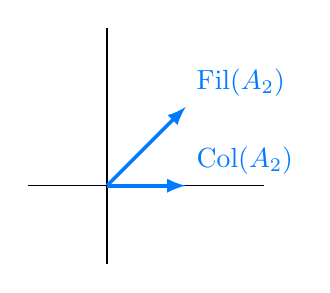
\begin{tikzpicture}[>=latex, baseline=(current bounding box.center)]
        \draw (-1,0) -- (2,0);
        \draw (0,-1) -- (0,2);
        \draw[lightblue, ->, line width=1.3] (0,0) -- (1,1) node[above right] {$\mathrm{Fil}(A_2)$};
        \draw[lightblue, ->, line width=1.3] (0,0) -- (1,0) node[above right] {$\mathrm{Col}(A_2)$};
    \end{tikzpicture}

    \item \lb{Sea $A$ una matriz $10\times 10$ que cumple $A^2=0$. Prueba que $\mathrm{Col}(A)\subseteq \mathrm{Nuc}(A)$ y en consecuencia, el rango de $A$ es menor o igual que 5.}

        Sea $v\in \mathrm{Col}(A)\longrightarrow \exists x\in \R^{10}:Ax=v$ 

        Por tanto: \[
            \underbrace{A(Ax)}_{A^2x=0}=Av,
        \] 
        es decir, $v$ es solución de  $Av=0\longrightarrow v \in \mathrm{Nuc}(A)$.

        Por el \textbf{teorema de la dimensión}, tenemos: \[
        \mathrm{dimCol}(A)+\mathrm{dimNuc}(A)=10.
        \]  
        Llamemos: \[
        \mathrm{dimCol}(A)=r\quad(\text{el rango de $A$}).
        \] 
        Entonces: \[
            \mathrm{dimNuc}(A)=10-r.
        \] 
        Dado que $\mathrm{Col}(A)\subseteq\mathrm{Nuc}(A)$, se cumple: \[
        r\le \mathrm{dimNuc}(A).
        \] 
        Sustituyendo $\mathrm{dimNuc}(A)$, se cumple: \[
        r\le \mathrm{dimNuc}(A).
        \] 
        Sustituyendo $\mathrm{dimNuc}(A)=10-r$, obtenemos: \[
        r\le 10-r\longrightarrow 2r\le 10\longrightarrow r\le 5.
        \] 
        Por lo tanto, el rango de $A$ es como máximo 5.
    \item \lb{Sea $A$ una matriz cuadrada invertible. Calcula una base para cada uno de los subespacios fundamentales de las matrices $A$ y $B=\begin{bmatrix} 
                A & A
    \end{bmatrix} $.} 

    \textbf{Subespacios fundamentales de $A$}

    Dado que $A$ es invertible:
    \begin{enumerate}[label=\arabic*)]
        \item $\mathrm{Col}(A)$:
            \begin{itemize}[label=\textbullet]
                \item Como $A$ es invertible, sus columnas forman una base de $\R^n$.
                \item Base: Las columnas de $A$.
            \end{itemize}
        \item $\mathrm{Fil}(A)$:
            \begin{itemize}[label=\textbullet]
                \item Dado que $A$ es invertible, sus filas abarcan también todo  $\R^n$.
                \item Base: Las filas de $A$.
            \end{itemize}
        \item $\mathrm{nuc}(A)$ ;
            \begin{itemize}[label=\textbullet]
                \item Dado que $A$ es invertible,  $Ax=0$ solo tiene la solución trivial  $x=0$.
                \item Base:  $\varnothing$ (dimensión 0).
            \end{itemize}
        \item $\mathrm{nuc}(A^\intercal)$:
            \begin{itemize}[label=\textbullet]
                \item Dado que $A$ es invertible,  $A^\intercal y=0$ también tiene solo la solución trivial $y=0$ 
                \item Base:  $\varnothing$ (dimensión 0).
            \end{itemize}
    \end{enumerate}
    \textbf{Subespacios fundamentales de $B=\begin{bmatrix} 
            A & A 
    \end{bmatrix} $} 

    La matriz $B$ tiene tamaño $n\times 2n$. Analices sus subespacios fundamentales:
    \begin{enumerate}[label=\arabic*)]
        \item $\mathrm{Col}(B)$:
            \begin{itemize}[label=\textbullet]
                \item Las columans de $B$ son combinaciones lineales de las columnas de $A$. Como $A$ es invertible, sus columnas ya abarcan todo  $\R^n$.
                \item Base: Las columnas de $A$.
            \end{itemize}
        \item $\mathrm{Fil}(B)$:
            \begin{itemize}[label=\textbullet]
                \item Las filas de $B$ son las mismas que las filas de $A$ duplicadas, pero no generan un espacio mayor que el de $A$.
                \item Base: Las filas de  $A$.
            \end{itemize}
        \item $\mathrm{Nuc}(B)$:
            \begin{itemize}[label=\textbullet]
                \item Resolviendo $Bx=0$, donde  $B=\begin{bmatrix} 
                        A & A 
                \end{bmatrix} $ :
                \[
                \begin{bmatrix} 
                    A & A 
                \end{bmatrix} \begin{bmatrix} 
                x_1\\ x_2 
                \end{bmatrix} =0\longrightarrow A(x_1+x_2)=0.
                \] 
                Como $A$ es invertible,  $x_1+x_2=0$, es decir, $x_1=-x_2$. Esto implica que: \[
                \begin{bmatrix} 
                x_1\\ x_2 
                \end{bmatrix} =\begin{bmatrix} 
                -x_2\\ x_2 
                \end{bmatrix} =x_2\begin{bmatrix} 
                -1\\ 1 
                \end{bmatrix} .
                \] 
            \item Base: $\left<(-1,1) \right>$.
            \end{itemize}
        \item $\mathrm{Nuc}(B^\intercal)$ :
            \begin{itemize}[label=\textbullet]
                \item Resolviendo $B^\intercal y=0$, donde: \[
                B^\intercal=\begin{bmatrix} 
                A^\intercal\\ A^\intercal 
                \end{bmatrix} .
                \] 
                Esto implica que: \[
                \begin{bmatrix} 
                A^\intercal\\ A^\intercal 
                \end{bmatrix} y=0\longrightarrow A^\intercal y_1=0\text{ y }A^\intercal y_2=0.
                \] 
                Como $A$ es invertible,  $A^\intercal y=0$ solo tiene la solución trivial. Por lo tanto, el espacio nulo a la izquierda es trivial.
            \item Base: $\varnothing$.
            \end{itemize}
    \end{enumerate}
    \item \lb{Sin calcular la matriz $A$, encuentra bases para sus cuatro subespacios fundamentales \[
    A=\begin{bmatrix} 
        1 & 0 & 0\\
        6 & 1 & 0\\
        9 & 8 & 1
    \end{bmatrix}\begin{bmatrix} 
        1 & 2 & 3 & 4\\
        0 & 1 & 2 & 3\\
        0 & 0 & 1 & 2
    \end{bmatrix}  
    \] } 
\item \lb{Halla una base del subespacio de $\R^4$ dado por el núcleo de $A$, donde \[
A=\begin{bmatrix} 
    3 & 0 & 1 & 2\\
    1 & 1 & 0 & 1 
\end{bmatrix} 
\]Comprueba que el vector $(1,1,1-2)$ pertenece a $\mathrm{Nuc}(A)$ y calcula sus coordenadas respecto de la base obtenida.}

    \begin{enumerate}[label=Paso \arabic*:]
        \item Calcular el núcleo de $A$

            El núcelo de  $A$ es el conjunto de vectores $x \in \R^4$ tales que $Ax=0$. Resolvemos el sistema homogéneo  $Ax=0$:  \[
            Ax=\begin{bmatrix} 
                3 & 0 & 1 & 2\\
                1 & 1 & 0 & 1
            \end{bmatrix} \begin{bmatrix} 
            x_1\\ x_2\\ x_3\\ x_4 
            \end{bmatrix} =\begin{bmatrix} 
            0\\ 0 
            \end{bmatrix} \longrightarrow \begin{cases}
                3x_1+x_3+2x_4=0\\
                x_1+x_2+x_4=0
            \end{cases}
            \] 
        \item Resolver el sistema

            De la segunda ecuación: \[
            x_2=-x_1-x_4.
            \] 
            Sustituyendo $x_2$ en la primera ecuación: \[
            3x_1+x_3+2x_4=0\longrightarrow x_3=-3x_1-2x_4.
            \] 
            Ahora expresamos $x$ en función de $x_1$ y $x_4$: \[
            x=\begin{bmatrix} 
            x_1\\ x_2\\x_3\\x_4 
            \end{bmatrix} =\begin{bmatrix} 
            x_1\\ -x_1-x_4\\-3x_1-2x_4\\x_4 
            \end{bmatrix}=x_1\begin{bmatrix} 
            1\\-1\\3\\0 
            \end{bmatrix}+x_4\begin{bmatrix} 
            0\\-1\\-2\\1 
            \end{bmatrix}.
            \] 
        \item Base del núcleo de $A$

            Los vectores generadores del núcleo son:  \[
            v_1=\begin{bmatrix} 
            1\\-1\\-3\\0 
            \end{bmatrix},\quad v_2=\begin{bmatrix} 
            0\\-1\\-2\\1 
            \end{bmatrix}.  
            \] 
            Por lo tanto, una base del núcleo de $A$ es:  \[
            \mathcal{B}_{\mathrm{Nuc}(A)}= <(1,-1,-3,-0),(0,-1,-2,1)>.
            \] 
        \item Verficiar que $(1,1,1,-2)\in \mathrm{Nuc}(A)$ 

            Sea $x=(1,1,1,-2)$. Comprobamos si  $Ax=0$:  \[
            Ax=\begin{bmatrix} 
                3 & 0 & 1 & 2\\
                1 & 1 & 0 & 1
            \end{bmatrix} \begin{bmatrix} 
            1\\1\\1\\-2 
            \end{bmatrix}=\begin{bmatrix} 
            3+1-4\\ 1+1-2 
            \end{bmatrix}=\begin{bmatrix} 
            0\\ 0 
            \end{bmatrix}.
            \] 
            Por lo tanto, $x \in \mathrm{Nuc}(A)$.
        \item Coordenadas de $(1,1,1,-2)$ respecto de la base $\mathcal{B}_{\mathrm{Nuc}(A)}$ 

            Queremos expresar $(1,1,1,-2)$ como combinación lineal de  $v_1$ y $v_2$: \[
                (1,1,1,-2)=c_1v_1+c_2v_2,
            \] donde: \[
            c_1\begin{bmatrix} 
            1\\-1\\-3\\0 
            \end{bmatrix}+c_2\begin{bmatrix} 
            0\\-1\\-2\\1 
            \end{bmatrix}=\begin{bmatrix} 
            1\\1\\1\\-2 
            \end{bmatrix}\longrightarrow \begin{cases}
                c_1=1\\
                -c_1-c_2=1\\
                -3c_1-2c_2=1\\
                c_2=-2
            \end{cases}.   
            \] 
            De la primera y cuarta ecuación: \[
            c_1=1,\quad c_2=-2.
            \] 
            Verificamos con las demás ecuaciones: \[
            \begin{array}{l}
                -1\cdot 1-1\cdot (-2)=-1+2=1\quad\lb{\checkmark}\\
                -3\cdot 1-2\cdot (-2)=-3+4=1\quad \lb{\checkmark} 
            \end{array}
            \] 
            Por lo tanto, las coordenadas de $(1,1,1,-2)$ respecto de la base son:  \[
                (1,1,1,-2)=1\cdot v_1-2\cdot v_2.
            \] 
    \end{enumerate}
\item \lb{Dadas las siguientes bases de $\R^4$ \[
\begin{array}{c}
    \mathcal{B}_1=\{v_1=(1,1,0,0),v_2=(0,1,0,0),v_3=(0,0,1,1),v_4=(0,0,0,1)\} \\
    \mathcal{B}_2=\{w_1=(1,2,0,0),w_2=(0,1,2,-1),w_3=(0,1,1,1),w_4=(0,1,2,0)\}
\end{array}
\]encuentra la matriz de cambio de base de $\mathcal{B}_1$ y $\mathcal{B}_2$ y la del cambio inverso. ¿Qué coordenadas tiene el vector $3v_1-v_3+2v_2$ con respecto a la base $\mathcal{B}_2$? ¿Qué coordenadas tiene el vector $3w_1-w_3+2w_2$ con respecto a la base $\mathcal{B}_1$?} 

\begin{enumerate}[label=Paso \arabic*:]
    \item Matriz de cambio de base de $\mathcal{B}_1$ a $\mathcal{B}_2$ 

        Sea $P_{\mathcal{B}_1\to \mathcal{B}_2}$ la matriz de cambio de base de $\mathcal{B}_1$ a $\mathcal{B}_2$. Para calcularla:
        \begin{enumerate}[label=\arabic*)]
            \item Expresamos cada vector $v_i \in \mathcal{B}_1$ como combinación lineal de los vectores $w_j\in \mathcal{B}_2$: \[
            v_i=c_1w_1+c_2w_2+c_3w_3+c_4w_4,
            \] y los coeficientes $c_1,c_2,c_3,c_4$ forman las columnas de $P_{\mathcal{B}_1\to \mathcal{B}_2}$.
        \item Esto equivale a resolver el sistema lineal: \[
        \begin{bmatrix} 
            w_1 & w_2 & w_3 & w_4 
        \end{bmatrix} \begin{bmatrix} 
         c_1\\ c_2\\ c_3\\ c_4
        \end{bmatrix} =v_i,\quad \text{para cada $v_i$.}
        \] 

        \end{enumerate}
        Definimos las matrices: \[
        W=\begin{bmatrix} 
            w_1 & w_2 & w_3 & w_4 
        \end{bmatrix} =\begin{bmatrix} 
            1 & 0 & 0 & 0\\
            2 & 1 & 1 & 1\\
            0 & 2 & 1 & 2\\
            0 & -1 & 1 & 0
        \end{bmatrix} ,\quad V=\begin{bmatrix} 
            v_1 & v_2 & v_3 & v_4 
        \end{bmatrix} =\begin{bmatrix} 
            1 & 0 & 0 & 0\\
            1 & 1 & 0 & 0\\
            0 & 0 & 1 & 0\\
            0 & 0 & 1 & 1
        \end{bmatrix} .
        \] 
        Resolvemos: \[
        P_{\mathcal{B}_1\to \mathcal{B}_2}=W^{-1}V.
        \] 
    \item Matriz de cambio de base inversa

        La matriz de cambio de base inversa, $P_{\mathcal{B}_2\to \mathcal{B}_1}$, es: \[
        P_{\mathcal{B}_2\to \mathcal{B}_1}=P_{\mathcal{B}_1\to \mathcal{B}_2}^{-1}.
        \] 
    \item Coordenadas del vector $3v_1-v_3+2v_2$ en la base $\mathcal{B}_2$ 
        \begin{enumerate}[label=\arabic*)]
            \item Escribimos el vector en $\mathcal{B}_1$ como: \[
            x=3v_1-v_3+2v_2=3\begin{bmatrix} 
            1\\ 1\\ 0\\ 0 
            \end{bmatrix}+2\begin{bmatrix} 
            0\\1\\0\\0 
            \end{bmatrix}  -\begin{bmatrix} 
            0\\0\\1\\1 
            \end{bmatrix}=\begin{bmatrix} 
            3\\5\\-1\\-1 
            \end{bmatrix}.  
            \] 
        \item Multiplicamos $P_{\mathcal{B}_1\to \mathcal{B}_2}$ por $x$ para encontrar las coordenadas en  $\mathcal{B}_2$ : \[
                [x]_{\mathcal{B}_2}=P_{\mathcal{B}_1\to \mathcal{B}_2}x.
        \] 
    \item Coordenadas del vector $3w_1-w_3+2w_2$ en la base $\mathcal{B}_1$ 
        \begin{enumerate}[label=\arabic*)]
            \item Escribimos el vector en $\mathcal{B}_2$ como: \[
            y=3w_1-w_3+2w_2=3\begin{bmatrix} 
            1\\2\\0\\0 
            \end{bmatrix} +2\begin{bmatrix} 
            0\\1\\2\\-1 
            \end{bmatrix} -\begin{bmatrix} 
            0\\1\\1\\1 
            \end{bmatrix} =\begin{bmatrix} 
            3\\6\\4\\-5 
            \end{bmatrix} .
            \] 
        \item Multiplicamos $P_{\mathcal{B}_2\to \mathcal{B}_1}$ por $y$ para encontrar las coordenadas en  $\mathcal{B}_1$: \[
                [y]_{\mathcal{B}_1}=P_{\mathcal{B}_2\to \mathcal{B}_1}y.
        \] 
        \end{enumerate}
        Calculamos las matrices $P_{\mathcal{B}_1\to \mathcal{B}_{2}}$ y $P_{\mathcal{B}_2\to \mathcal{B}_1}$: \[
        P_{\mathcal{B}_1\to \mathcal{B}_2}=W^{-1}\cdot V=\begin{bmatrix} 
            1 & 0 & 0 & 0\\
            -4 & 2 & -1 & -1\\
            -4 & 2 & -1 & 0\\
            6 & -3 & 2 & 1
        \end{bmatrix} \begin{bmatrix} 
            1 & 0 & 0 & 0\\
            1 & 1 & 0 & 0\\
            0 & 0 & 1 & 0\\
            0 & 0 & 1 & 1
        \end{bmatrix} =\begin{bmatrix} 
            1 & 0 & 0 & 0\\
            -2 & 2 & -2 & -1\\
            -2 & 2 & -1 & 0\\
            3 & -3 & 3 & 1
        \end{bmatrix} 
        \] 
        \[
        P_{\mathcal{B}_2\to \mathcal{B}_1}=P_{\mathcal{B}_1\to \mathcal{B}_2}^{-1}=\begin{bmatrix} 
            1 & 0 & 0 & 0\\
            1 & 1 & 1 & 1\\
            0 & 2 & 1 & 2\\
            0 & -3 & 0 & -2
        \end{bmatrix} 
        \] 
        \[
       \begin{array}{l}
           [x]_{\mathcal{B}_2}=P_{\mathcal{B}_1\to \mathcal{B}_2}x=\begin{bmatrix} 
               1 & 0 & 0 & 0\\
               -2 & 2 & -2 & -1\\
               -2 & 2 & -1 & 0\\
               3 & -3 & 3 & 1
           \end{bmatrix} \begin{bmatrix} 
           3\\5\\-1\\-1 
           \end{bmatrix}=\begin{bmatrix} 
           3\\7\\5\\-10 
           \end{bmatrix} \\
           \left[ y \right] _{\mathcal{B}_1}=P_{\mathcal{B}_2\to \mathcal{B}_1}y=\begin{bmatrix} 
               1 & 0 & 0 & 0\\
               1 & 1 & 1 & 1\\
               0 & 2 & 1 & 2\\
               0 & -3 & 0 & -2
           \end{bmatrix} \begin{bmatrix} 
           3\\6\\4\\-5 
           \end{bmatrix} =\begin{bmatrix} 
           3\\8\\6\\-8 
           \end{bmatrix}\\ 
       \end{array} 
        \] 
        \end{enumerate}
\end{enumerate}
\item \lb{Calcula una base y unas ecuaciones implícitas de $U+V$, donde  \[
\begin{array}{c}
    U=\left<(1,2,3,4,5),(5,4,3,2,1),(-1,0,1,2,3) \right>\\
    V=\left\{ (x,y,z,r,s): \begin{array}{l}
        3x+r=2y\\
        3x+s=2y
    \end{array} \right\} 
\end{array}
\] } 
\begin{enumerate}[label=Paso \arabic*:]
    \item Determinar una base para $U$

        El subespacio  $U$ está generado por los vectores: \[
        U=\left<(1,2,3,4,5),(5,4,3,2,1),(-1,0,1,2,3) \right>.
        \] 
        Escribimos estos vectores como filas de una matriz y determinamos las filas linealmente independientes: \[
\begin{aligned}
        M_U=\begin{bmatrix} 
            1 & 2 & 3 & 4 & 5\\
            5 & 4 & 3 & 2 & 1\\
            -1 & 0 & 1 & 2 & 3
        \end{bmatrix}&\xrightarrow[F_3\to F_3+F_1]{F_2\to F_2-5F_1}\begin{bmatrix} 
            1 & 2 & 3 & 4 & 5\\
            0 & -6 & -12 & -18 & -24\\
            0 & 2 & 4 & 6 & 8
        \end{bmatrix}\xrightarrow{F_2\to -\frac{1}{3} F_2}\begin{bmatrix} 
            1 & 2 & 3 & 4 & 5\\
            0 & 2 & 4 & 6 & 8\\
            0 & 2 & 4 & 6 & 8\\
        \end{bmatrix}\\ & \xrightarrow{F_3\to F_3-F_2}\begin{bmatrix} 
            1 & 2 & 3 & 4 & 5\\
            0 & 2 & 4 & 6 & 8\\
            0 & 0 & 0 & 0 & 0
        \end{bmatrix} \xrightarrow{F_{3}\to \frac{1}{2} F_3} \begin{bmatrix} 
            1 & 2 & 3 & 4 & 5\\
            0 & 1 & 2 & 3 & 4\\
            0 & 0 & 0 & 0 & 0
        \end{bmatrix}  .
\end{aligned}
        \] 

        Por lo tanto: \[
        \mathcal{B}_U=\{(1,2,3,4,5),(0,1,2,3,4)\} 
        \] 
    \item Determinar una base para $V$

        El subespacio  $V$ etá definido por las ecuaciones:  \[
        \begin{array}{l}
            3x+r=2y\\
            3x+s=2y
        \end{array}
        \] 
        Resolvemos el sistema para encontrar las relaciones entr las variables: \[
        r=2y-3x,\quad s=2y-3x.
        \] 
        Entonces, $V$ está parametrizado como:  \[
            (x,y,z,r,s)=(x,y,z,2y-3,2y-3).
        \] 
        Podemos expresar los vectores de $V$ en términos de  $x,y,z$:  \[
            (x,y,z,r,s)=x(1,0,0,-3,-3)+y(0,1,0,2,2)+z(0,0,1,0,0).
        \] 
        Por lo tanto, una base de $V$ es:  \[
        \mathcal{B}_V=\{(1,0,0,-3,-3),(0,1,0,2,2),(0,0,1,0,0)\} .
        \] 
    \item Determinar una base para $U+V$

        Los vectores  $U+V$ son combinaciones lineales de las bases de  $U$ y $V$. Por lo tanto, los generadores de $U+V$ son las uniones de las bases de  $U$ y $V$:  \[
        \mathcal{S}=\{(1,2,3,4,5),(5,4,3,2,1),(-1,0,1,2,3),(1,0,0,-3,-3),(0,0,1,0,0)\} .
        \] 
        Escribimos estos vectores como filas de una matriz: \[
        M_{U+V}=
        \begin{bmatrix} 
            1 & 2 & 3 & 4 & 5\\
            5 & 4 & 3 & 2 & 1\\
            -1 & 0 & 1 & 2 & 3\\
            1 & 0 & 0 & -3 & -3\\
            0 & 1 & 0 & 2 & 2\\
            0 & 0 & 1 & 0 & 0
        \end{bmatrix} .
        \] 
        Reducimos $M_{U+V}$ por filas para encontrar una base para $U+V$.  \[
        \begin{aligned}
        \begin{bmatrix} 
            1 & 2 & 3 & 4 & 5\\
            5 & 4 & 3 & 2 & 1\\
            -1 & 0 & 1 & 2 & 3\\
            1 & 0 & 0 & -3 & -3\\
            0 & 1 & 0 & 2 & 2\\
            0 & 0 & 1 & 0 & 0
        \end{bmatrix}&\xrightarrow[\begin{subarray}{l}
            F_3\to F_3+F_1\\
            F_4\to F_4-F_1
        \end{subarray}]{F_2\to F_2-5F_1}
        \begin{bmatrix} 
            1 & 2 & 3 & 4 & 5 \\
            0 & -6 & -12 & -18 & -24\\
            0 & 2 & 4 & 6 & 8\\
            0 & -2 & -3 & -7 & -8\\
            0 & 1 & 0 & 2 & 2\\
            0 & 0 & 1 & 0 & 0
        \end{bmatrix}\xrightarrow[F_3\leftrightarrow F_6]{F_2\leftrightarrow F_5} \begin{bmatrix} 
            1 & 2 & 3 & 4 & 5\\
            0 & 1 & 0 & 2 & 2\\
            0 & 0 & 1 & 0 & 0\\
            0 & -2 & -3 & -7 & -8\\
            0 & -6 & -12 & -18 & -24\\
            0 & 2 & 4 & 6 & 8
        \end{bmatrix}\\
& \xrightarrow[\begin{subarray}{l}
            F_5\to F_5+6F_2\\
            F_6\to F_6-2F_2
        \end{subarray}]{F_4\to F_4+2F_2}\begin{bmatrix} 
            1 & 2 & 3 & 4 & 5\\
            0 & 1 & 0 & 2 & 2\\
            0 & 0 & 1 & 0 & 0\\
            0 & 0 & -3 & -3 & -4\\
            0 & 0 & -12 & -6 & -12\\
            0 & 0 & 4 & 2 & 4
        \end{bmatrix} \xrightarrow[\begin{subarray}{l}
            F_5\to F_5+12F_3\\
            F_6\to F_6-4F_3
        \end{subarray}]{F_4\to F_4+3F_3}\begin{bmatrix} 
            1 & 2 & 3 & 4 & 5\\
            0 & 1 & 0 & 2 & 2\\
            0 & 0 & 1 & 0 & 0\\
            0 & 0 & 0 & -3 & -4\\
            0 & 0 & 0 & -6 & -12\\
            0 & 0 & 0 & 2 & 4
        \end{bmatrix}\\
& \xrightarrow[F_5\leftrightarrow F_6]{F_4\leftrightarrow F_5}\begin{bmatrix} 
            1 & 2 & 3 & 4 & 5\\
            0 & 1 & 0 & 2 & 2\\
            0 & 0 & 1 & 0 & 0\\
            0 & 0 & 0 & 1 & 2\\
            0 & 0 & 0 & -3 & -4\\
            0 & 0 & 0 & 0 & -4
        \end{bmatrix} \xrightarrow[F_6\to -\frac{1}{4} F_6]{F_5\to F_5+3F_4} \begin{bmatrix} 
            1 & 2 & 3 & 4 & 5\\
            0 & 1 & 0 & 2 & 2\\
            0 & 0 & 1 & 0 & 0\\
            0 & 0 & 0 & 1 & 2\\
            0 & 0 & 0 & 0 & 2\\
            0 & 0 & 0 & 0 & 1
        \end{bmatrix}\\
& \xrightarrow[F_5\to \frac{1}{2} F_5]{F_6\to F_6-\frac{1}{2} F_5}\begin{bmatrix} 
            1 & 2 & 3 & 4 & 5\\
            0 & 1 & 0 & 2 & 2\\
            0 & 0 & 1 & 0 & 0\\
            0 & 0 & 0 & 1 & 2\\
            0 & 0 & 0 & 0 & 1\\
            0 & 0 & 0 & 0 & 0
        \end{bmatrix}\xrightarrow[\begin{subarray}{l}
F_2\to F_2-2F_5\\
F_4\to F_4-2F_5
\end{subarray}]{F_1\to F_1-5F_5}\begin{bmatrix} 
            1 & 2 & 3 & 4 & 0\\
            0 & 1 & 0 & 2 & 0\\
            0 & 0 & 1 & 0 & 0\\
            0 & 0 & 0 & 1 & 0\\
            0 & 0 & 0 & 0 & 1\\
            0 & 0 & 0 & 0 & 0
        \end{bmatrix}\\
& \xrightarrow[F_2\to F_2-2F_4]{F1\to F_1-4F_4}\begin{bmatrix} 
            1 & 2 & 3 & 0 & 0\\
            0 & 1 & 0 & 0 & 0\\
            0 & 0 & 1 & 0 & 0\\
            0 & 0 & 0 & 1 & 0\\
            0 & 0 & 0 & 0 & 1\\
            0 & 0 & 0 & 0 & 0
        \end{bmatrix}\xrightarrow{F_1\to F_1-3F_3}\begin{bmatrix} 
            1 & 2 & 0 & 0 & 0\\
            0 & 1 & 0 & 0 & 0\\
            0 & 0 & 1 & 0 & 0\\
            0 & 0 & 0 & 1 & 0\\
            0 & 0 & 0 & 0 & 1\\
            0 & 0 & 0 & 0 & 0
        \end{bmatrix}\\
& \xrightarrow{F_1\to F_1-2F_2}\begin{bmatrix} 
            1 & 0 & 0 & 0 & 0\\
            0 & 1 & 0 & 0 & 0\\
            0 & 0 & 1 & 0 & 0\\
            0 & 0 & 0 & 1 & 0\\
            0 & 0 & 0 & 0 & 1\\
            0 & 0 & 0 & 0 & 0
        \end{bmatrix}.
        \end{aligned}
        \]  
    \item Determinar las ecuaciones implícitas para $U+V$

        Si  $\mathrm{dim}(U+V)=k$, el espacio nulo de $M_{U+V}$ tiene dimensión $5-k$. Las ecuaciones implícitas de $U+V$ son las relaciones lineales que definen el espacio nulo de $M_{U+V}$.

\textbf{Resultados}
\begin{enumerate}[label=\arabic*)]
\item Base de $U+V$:

La matriz tiene rango completo $(\mathrm{dim}(U+V)=5)$. Por lo tanto, los vectores generadores $(1,2,3,4,5),(5,4,3,2,1)$, $(-1,0,1,2,3),(1,0,0,-3,-3)$, y $(0,1,0,2,2)$ forman una base para $U+V$.
\item Ecuaciones implícitas de $U+V$:

Como el espacio tiene dimensión completa $(\mathrm{dim}(U+V)=5)$, no hay restricciones adicionales, y el espacio es $\R^5$. Por lo tanto, no hay ecuaciones implícitas no triviales para $U+V$.
\end{enumerate}
\end{enumerate}
\end{enumerate}
\end{document}
